
Se desea trabajar con series temporales sobre mediciones climatológicas. 
En concreto, se eligen las variables de temperatura del aire, humedad relativa y presión atmosférica en la superficie.
Dichas variables son estudiadas con frecuencia horaria, en el intervalo comprendido entre el 1 de marzo de 2023 y el 28 de febrero de 2025.

Es relevante el uso de datos en un período múltiplo del año, para asegurar que se capturan las variaciones estacionales y que el conjunto de datos está suficientemente equilibrado.

\section{Fuentes de los datos}

Se han empleado 2 fuentes para recopilar las mediciones: 
\begin{itemize}
    \item \textbf{Grafcan}: Cartográfica de Canarias, S.A. es una empresa pública de la Comunidad Autónoma de Canarias. Dispone de una red de estaciones meteorológicas cuyas
    mediciones son accesibles mediante una API REST de acceso gratuito previa solicitud de una clave\cite{grafcan_sensores}. 
    \item \textbf{Open-Meteo}: API pública de código abierto que proporciona datos de múltiples proveedores de meteorología. Este servicio no dispone de estaciones de medición
    propias, sino que recopila pronósticos de diferentes modelos de predicción climatológica. 

    Se emplea la API de predicciones pasadas\cite{open_meteo_api}. Se seleccionan los modelos ICON Global del servicio meteorológico alemán (DWD) y el modelo ARPEGE Europe de Météo-France. Ambos modelos se actualizan cada 3 horas. 
    Se explora la posibilidad de emplear as predicciones del modelo HAROME de la AEMET, pero no están disponibles de forma pública
\end{itemize}

Se eligen 4 ubicaciones de la isla de Tenerife con distintas características climáticas para el conjunto de entrenamiento y evaluación:
\begin{itemize}
    \item \textbf{San Cristóbal de La Laguna 1}: La Cuesta, 35 metros de altitud.
    \item \textbf{San Cristóbal de La Laguna 2}: La Punta del Hidalgo, 54m.
    \item \textbf{La Orotava}: Camino de Chasna, 812m.
    \item \textbf{Arona}: Punta de Rasca, 25m.
\end{itemize}

Así mismo, se escogen 2 ubicaciones para el conjunto de test, nunca vistas en el ajuste del modelo:
\begin{itemize}
    \item \textbf{Garachico}: La Cuesta, 35 metros de altitud.
    \item \textbf{Santa Cruz de Tenerife}: Camino de Chasna, 812m.
\end{itemize}

Las ubicaciones han sido elegidas al contar con estaciones de medición de Grafcan.
Sus posiciones se muestran en la Figura \ref{mapa_estaciones}, señaladas en rojo. De izquierda a derecha: Arona, La Orotava y San Cristóbal de La Laguna.

\begin{figure}[htb]
   \centering
   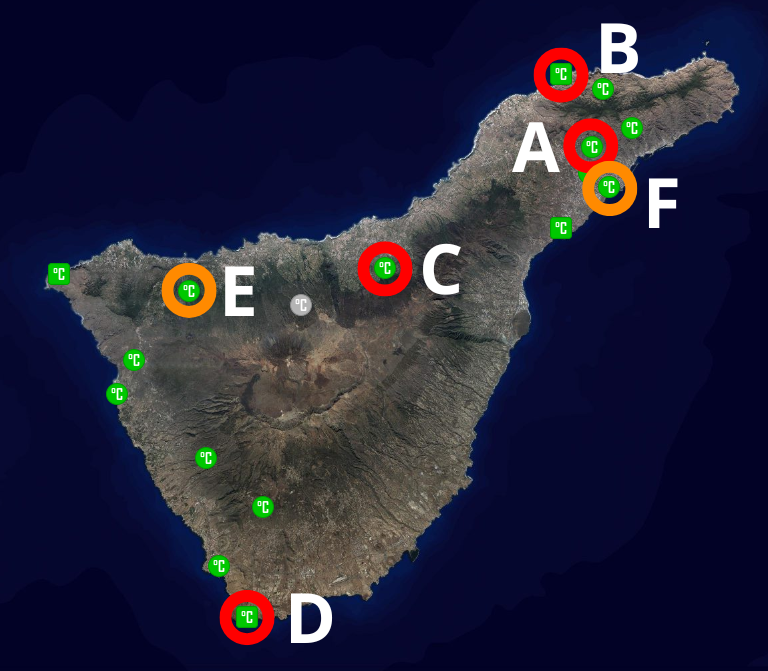
\includegraphics[width=0.6\linewidth]{images/mapa_estaciones}
   \caption{Mapa de las estaciones climatológicas Grafcan empleadas.}
   \label{mapa_estaciones}
\end{figure}

Inicialmente se valoró emplear las estaciones correspondientes a Los Cristianos, Santiago del Teide o la Punta de Teno, pero fueron descartadas por dos motivos: 
se detectó que existían períodos prolongados con datos faltantes en las mediciones de Grafcan. Algunas de ellas también exhibían poca correlación entre las mediciones
del servicio Grafcan y las de Open-Meteo, lo que podría afectar la calidad de los datos.

\bigskip

\section{Proceso de adquisición}

Para automatizar la adquisición de datos, se emplea la herramienta de ---- node-red. En dicha herramienta se desarrollan dos panelea, uno para cada fuente de datos. 
Así mismo, dentro de cada panel se desarrollan dos flujos, uno para la adquisición de datos en un intervalo dado, y otro para la adquisición de datos en tiempo real.


Se estudian distintas alternativas para el almacenamiento de los datos.
Se opta por emplear TimescaleDB, una extensión del popular sistema PostgreSQL
de bases de datos relacionales, especialmente adaptada para el manejo de series temporales. 

